\begin{frame}
\begin{figure}
%\centering
%\begin{tabular}{c}
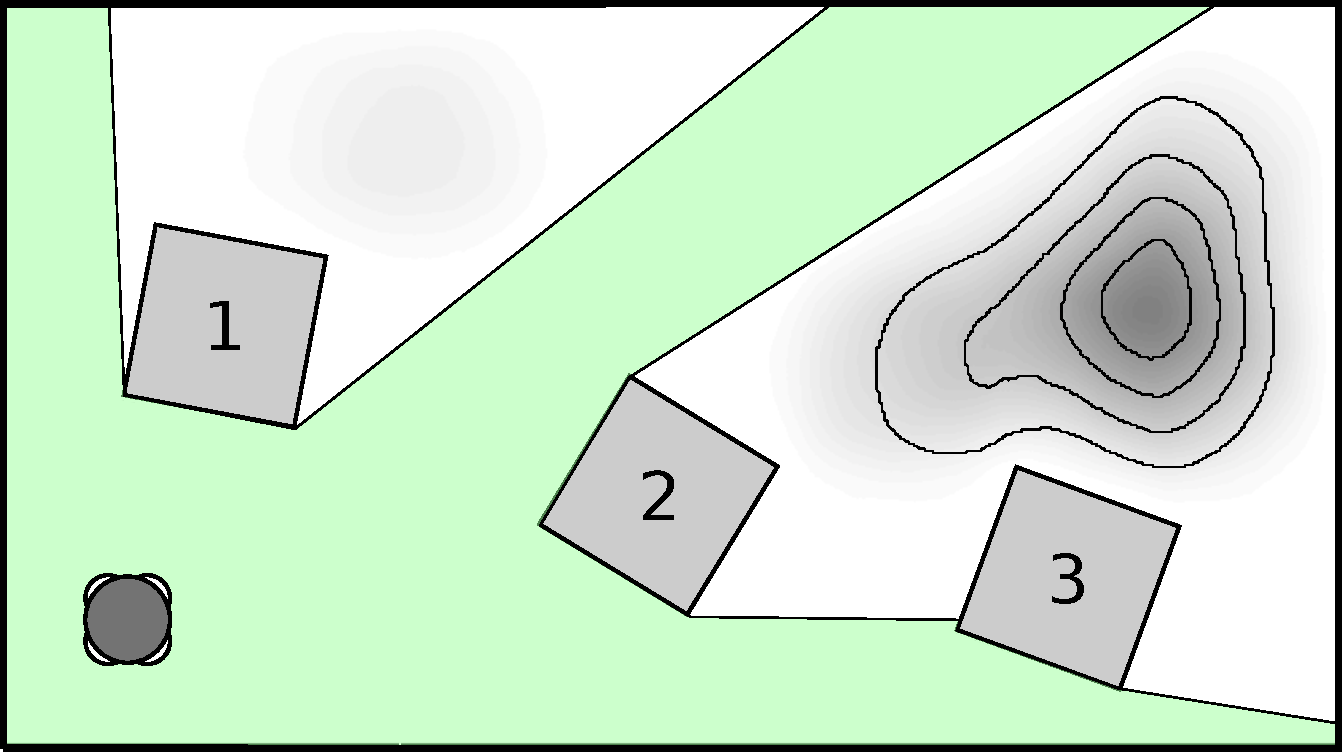
\includegraphics[height=1in]{random_block_marg}
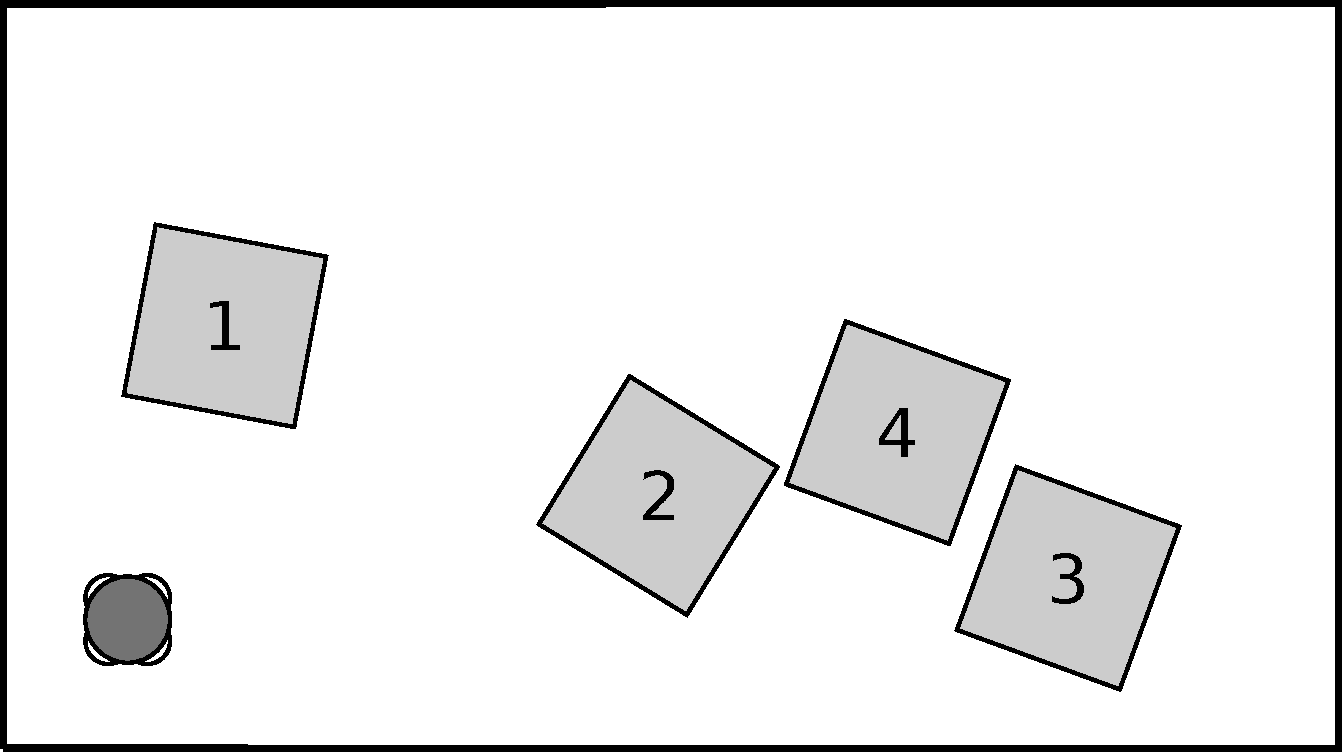
\includegraphics[height=1in]{random_block}
%\end{tabular}
\end{figure}
Here, the explorer knows that 
there are four identical boxes scattered within a
room of known dimensions, three of which he can see.
Based on allowable configurations 
of the missing block (blocks can not intersect, 
unseen blocks can not lie in known free space), the
explorer can compute, at each point in the shadow region,
the probability that that point is covered by an obstacle.
\end{frame}
